\documentclass[11pt]{article}

\usepackage[review]{acl}
\usepackage{times}
\usepackage{latexsym}
\usepackage[T1]{fontenc}
\usepackage[utf8]{inputenc}
\usepackage{microtype}
\usepackage{graphicx}
\usepackage{booktabs}
\usepackage{amsmath}
\usepackage{multirow}

\title{Match the Reference Frame: When Speaker Normalization Helps or Hurts Speech Emotion Recognition}

\author{Anonymous COLING 2027 Submission}

\begin{document}
\maketitle

\begin{abstract}
Speaker normalization is widely used in speech emotion recognition (SER) to suppress speaker-dependent variability, implicitly treating stable speaker characteristics as nuisance.
We argue that this assumption is conditional: whether speaker baseline information should be removed depends on the reference frame of the prediction target.
We decompose prosodic features into speaker centers and within-speaker deviations, decompose continuous affect targets analogously, and introduce a controlled intervention that continuously varies the amount of between-speaker target structure while keeping utterances, splits, and models fixed.
On MSP-Podcast, a six-attribute interpretable prosody representation yields strongly negative Relative-minus-Absolute slopes for Arousal and Dominance under speaker-cluster bootstrap; at the pure within-speaker endpoint, Relative significantly outperforms Absolute, while restoring speaker centers in a Hybrid representation is strongly beneficial for raw targets.
Semantically matched Pitch+Rate experiments on IEMOCAP preserve the same direction but are low-powered with only ten speakers.
Crucially, the same target-reference effect is significant when reference frames are constructed directly in frozen WavLM-large embeddings at layers 12 and 24.
Finally, unlabeled enrollment makes the effect practical: with 20 utterances, six-feature K-shot Hybrid improves over Absolute by 0.039 CCC for Arousal and 0.032 for Dominance; with 50 utterances it is within 0.0044/0.0037 CCC of the oracle Hybrid.
The results support a simple principle: representation reference frame should match target reference frame.
\end{abstract}

\section{Introduction}

Speech conveys affect together with many stable and slowly varying speaker characteristics.
Speakers differ in habitual pitch, loudness, speaking rate, voice quality, physiology, accent, and expressive style.
A long-standing response in speech emotion recognition (SER) is therefore to normalize away speaker variability or learn speaker-invariant representations.
Classical approaches estimate speaker-specific statistics and transform an utterance relative to a speaker baseline \citep{busso2013normalization,mariooryad2014compensating,bone2012arousal,bone2014arousal}; more recent systems suppress or compensate speaker information inside learned speech representations \citep{gat2022speaker}.
The underlying intuition is clear: if emotion is a transient state and speaker identity is stable, stable speaker information should be nuisance.

This intuition is often useful, but it does not specify what the target means.
Continuous affect labels are population-level annotations, and their variation can contain both within-speaker changes and stable between-speaker differences.
Two speakers can differ not only in acoustic baselines but also in average annotation values, expressive range, or how their behavior is mapped to population-level scales.
In such a setting, removing all stable speaker information can discard information that is predictive of the target.
Conversely, if the prediction target is explicitly defined as how this person differs from their own typical state, speaker baseline information is nuisance by construction.

We therefore treat speaker normalization as a \emph{reference-frame choice}.
Let an utterance-level acoustic representation for speaker $s$ and utterance $u$ be
\begin{equation}
    \mathbf{x}_{s,u} = \boldsymbol{\mu}_s + \boldsymbol{\delta}_{s,u},
\end{equation}
where $\boldsymbol{\mu}_s$ is a stable speaker center and $\boldsymbol{\delta}_{s,u}$ is a within-speaker deviation.
An Absolute representation uses $\mathbf{x}_{s,u}$; a Relative representation uses $\mathbf{x}_{s,u}-\boldsymbol{\mu}_s$; and a Hybrid representation concatenates the deviation with the center.
The target can be decomposed analogously,
\begin{equation}
    y_{s,u} = \bar{y}_s + \epsilon_{s,u},
\end{equation}
with a between-speaker component $\bar{y}_s$ and a within-speaker residual $\epsilon_{s,u}$.

This decomposition leads to our central hypothesis:
\begin{quote}
\textbf{Representation reference frame should match target reference frame.}
\end{quote}
If the target is dominated by within-speaker deviations, Relative features should be advantageous.
As the target contains more stable between-speaker structure, the advantage of Relative should diminish and correctly aligned speaker-center information can become useful.

Prior work shows both sides of this design choice.
Speaker normalization can improve categorical and continuous affect prediction \citep{busso2013normalization,dang2016factor,gat2022speaker}, while personalization, enrollment, and speaker-aware modeling can also improve SER \citep{triantafyllopoulos2024enrolment,shi2025speaker}.
Our question is not whether either strategy can work.
Instead, we ask \emph{when} the two apparently opposing strategies should help.
We test this by manipulating target reference frame directly rather than comparing unrelated datasets or models.

We first use low-dimensional prosody to establish an intuitive state--trait reversal: speaker-relative pitch improves categorical emotion recognition but strongly degrades gender decoding across ESD, MEAD, and RAVDESS.
We then move to continuous Arousal and Dominance.
On MSP-Podcast, we interpolate the target between a pure within-speaker residual and the raw population-level label while keeping acoustic inputs, speakers, folds, and models fixed.
The Relative-minus-Absolute performance difference decreases strongly as between-speaker target structure increases.
The effect persists when six interpretable prosodic attributes are combined and under both linear and quadratic Ridge models.

We then test mechanism rather than correlation.
A speaker-center permutation intervention preserves the marginal center distribution but assigns centers to the wrong speakers.
The large raw-target Hybrid benefit collapses under this intervention, and the true-versus-permuted gap nearly vanishes after within-speaker target centering.
We also move beyond hand-engineered prosody: constructing Absolute, Relative, and Hybrid reference frames directly in frozen WavLM-large embeddings reproduces the target-reference effect on IEMOCAP.
Finally, fixed-pool K-shot experiments show that the required speaker centers can be estimated from unlabeled enrollment speech rather than oracle access to a speaker's full history.

Our contributions are:
\begin{enumerate}
    \item a unified reference-frame formulation connecting speaker normalization and between/within-speaker target decomposition;
    \item a controlled target intervention that changes only target reference frame while keeping data and model family fixed;
    \item speaker-cluster inference over 1,915 MSP speakers, including a six-attribute interpretable representation and a speaker-center identity intervention;
    \item a learned-representation generalization in frozen WavLM-large embedding space; and
    \item a fixed-pool, unlabeled K-shot analysis showing that moderate enrollment recovers most of the practical speaker-center benefit.
\end{enumerate}

\section{Related Work}

\subsection{Speaker normalization and relative prosody}

Speaker normalization has a long history in affective speech processing.
Prosodic features scored relative to speaker-specific references can improve robustness, including cross-corpus arousal estimation \citep{bone2012arousal,bone2014arousal}.
Iterative normalization and compensation methods likewise reduce speaker and lexical variability for emotion recognition \citep{busso2013normalization,mariooryad2014compensating}.
For continuous emotion prediction, \citet{dang2016factor} explicitly decompose the acoustic feature space into speaker- and emotion-related subspaces and report improved arousal prediction after speaker normalization.
The same nuisance-removal motivation extends to learned representations: \citet{gat2022speaker} adversarially suppress speaker information for SSL-based SER, while \citet{ruggiero2025eta} linearly decompose WavLM representations into speaker-specific and speaker-independent components for content-driven speech tasks.

These studies establish that removing stable speaker variation can improve generalization.
Our question is different.
We do not introduce a new normalizer or claim that speaker invariance is universally desirable.
Instead, we manipulate how much stable between-speaker structure is present in the \emph{target} while holding utterances, acoustic inputs, folds, and model family fixed, and test whether the preferred representation changes accordingly.

\subsection{Personalization and speaker-aware affect modeling}

A complementary line of work explicitly retains or exploits speaker information.
Unsupervised personalization can improve affect recognition when speakers differ systematically in affect expression \citep{sridhar2022personalization}.
Pretrained encoders can be personalized with speaker-specific adaptation \citep{tran2023personalized}, and enrollment has been studied both for accuracy and individual-level fairness \citep{triantafyllopoulos2024enrolment}.
Recent systems also learn explicitly speaker-aware emotion representations \citep{shi2025speaker}, while inference-only speaker adaptation has been used to calibrate SER predictions to an unseen speaker's vocal range \citep{lachut2025inference}.
Speaker embeddings themselves can contain emotion-relevant structure \citep{ulgen2024emotional}.

Normalization and personalization are therefore not contradictory empirical findings.
They optimize different uses of speaker information.
Our reference-frame account predicts both: stable speaker information is nuisance for a within-person target but can be signal for a population-level target containing between-speaker structure.

\subsection{Between- and within-speaker variation}

Speech production exhibits substantial between- and within-speaker variation even for basic temporal properties \citep{jacewicz2010tempo,quene2008multilevel}.
Affective speech work has also modeled systematic speaker-dependent differences.
For example, \citet{grimm2006modeling} describe speaker-specific emotion-expression bias and amplification, separating a speaker's neutral location from the range over which that speaker expresses emotion.
These results motivate treating speaker means and within-speaker deviations as distinct statistical objects rather than assuming that one is merely a noisier version of the other.

Our study applies this distinction symmetrically to predictors and targets.
The key intervention is not only to estimate a speaker reference, but to construct a controlled family of targets that moves from a purely within-speaker residual to the original population-level label.
This makes it possible to test reference-frame matching directly.

\subsection{Positioning of the present work}

The closest prior literature contains the main ingredients separately: speaker-normalized continuous affect prediction \citep{dang2016factor}, explicit speaker-dependent affect baselines \citep{grimm2006modeling}, speaker-invariant SSL representations \citep{gat2022speaker,ruggiero2025eta}, and enrollment-based or speaker-aware personalization \citep{triantafyllopoulos2024enrolment,shi2025speaker}.
Our contribution is an explanatory test connecting these directions.
We ask whether the utility of normalization changes as a function of target reference frame itself.
We then test that mechanism with correct-versus-permuted speaker centers, speaker-cluster inference, frozen WavLM embeddings, and unlabeled K-shot reference estimation.
Thus the contribution is a reference-frame account and controlled evidence for it, rather than a claim to invent speaker normalization or personalization.

\section{Method}

\subsection{Acoustic reference frames}

For each acoustic feature vector $\mathbf{x}_{s,u}$, we estimate a speaker center $\boldsymbol{\mu}_s$ using coordinate-wise medians.
We evaluate three representations:
\begin{align}
    \textsc{Absolute}_{s,u} &= \mathbf{x}_{s,u},\\
    \textsc{Relative}_{s,u} &= \mathbf{x}_{s,u}-\boldsymbol{\mu}_s,\\
    \textsc{Hybrid}_{s,u} &= [\mathbf{x}_{s,u}-\boldsymbol{\mu}_s;\boldsymbol{\mu}_s].
\end{align}
Relative removes the stable center from the model input.
Hybrid preserves an explicit decomposition into deviation and center rather than requiring the model to recover that decomposition implicitly.

Our full interpretable representation contains six utterance-level attributes: pitch level $12\log_2(F0_{\mathrm{median}})$, F0 variability in semitones, speech loudness, log phoneme articulation rate, pause ratio, and voiced ratio.
For cross-corpus confirmation between MSP-Podcast and IEMOCAP, we restrict the main hand-engineered comparison to Pitch+Speaking Rate because their semantics are aligned across corpora.
We exclude IEMOCAP loudness from the main claim after a provenance sensitivity showed that alternative physically interpretable reconstructions change the result.

\subsection{Target reference-frame intervention}

Let $\bar{y}_s$ be the speaker mean target and $\epsilon_{s,u}=y_{s,u}-\bar{y}_s$ the within-speaker residual.
We define a continuum
\begin{equation}
    y^{(\lambda)}_{s,u} = \epsilon_{s,u}+\lambda\bar{y}_s,\qquad \lambda\in[0,1].
\end{equation}
At $\lambda=0$, the target is purely within-speaker.
At $\lambda=1$, the original raw target is recovered.
Importantly, changing $\lambda$ does not alter the acoustic inputs, speaker identities, folds, or model family.

Our primary statistic is the slope of
\begin{equation}
    \Delta(\lambda)=\mathrm{CCC}(\textsc{Relative})-\mathrm{CCC}(\textsc{Absolute})
\end{equation}
as a function of $\lambda$.
The reference-frame hypothesis predicts a negative slope.
We also inspect the pure within-speaker endpoint $\Delta(0)$ and the raw-target Hybrid benefit.

\subsection{Speaker-center identity intervention}

A Hybrid gain could arise merely from adding extra center-valued dimensions rather than from the correct speaker-center assignment.
We therefore derange speaker centers across speakers while preserving the marginal center distribution.
Each utterance keeps its Relative deviation, but the appended center belongs to another speaker.
If center utility reflects true target alignment, true-center Hybrid should outperform permuted-center Hybrid for raw targets and the difference should collapse after target centering.

\subsection{Unlabeled K-shot enrollment}

Oracle speaker centers use all available utterances and are not a deployable assumption.
For practical reference estimation, we reserve a fixed pool of 50 unlabeled utterances per eligible MSP speaker before downstream modeling.
For $K\in\{1,2,5,10,20,50\}$, the K-shot center is the coordinate-wise median of a nested prefix of that reserve.
All K values use identical downstream train/test rows within a seed, so performance changes cannot be caused by changing evaluation samples.
We compare Absolute, K-shot Hybrid, and a full-speaker marginal-oracle Hybrid.

\subsection{Frozen WavLM reference frames}

To test whether the mechanism is specific to hand-engineered prosody, we repeat the intervention in learned representation space using frozen WavLM-large \citep{chen2022wavlm}.
For IEMOCAP utterances, we pool hidden representations and construct speaker centers directly in the 1024-dimensional embedding space.
We evaluate layers 12 and 24, constructing Absolute, Relative, and Hybrid embeddings exactly as above.
No WavLM parameters are fine-tuned.

\subsection{Models and inference}

Continuous affect experiments use Ridge regression with $\alpha=1$.
The main interpretable analysis includes Linear Ridge and a Quadratic Ridge obtained by degree-2 expansion followed by standardization.
Evaluation uses Concordance Correlation Coefficient (CCC) \citep{lin1989ccc} with equal speaker weighting.
Folds are speaker-disjoint.

Inference treats speakers, not folds or random seeds, as the independent unit.
We use 5,000 speaker-cluster bootstrap replicates for the main target-reference analyses.
This correction matters on IEMOCAP: with only ten speakers, hand-engineered Pitch+Rate slope means remain negative but their cluster confidence intervals cross zero.
We therefore describe IEMOCAP hand-engineered results as directionally consistent external evidence rather than independent significance.

\section{Experimental Setup}

\paragraph{MSP-Podcast.}
MSP-Podcast is a large naturalistic emotional speech corpus with categorical and continuous Valence, Arousal, and Dominance annotations \citep{lotfian2019msp,busso2026msppodcast}.
The principal controlled analyses contain 197,014 utterances from 1,915 speakers after feature and label filtering.
The fixed-pool six-feature K-shot analysis additionally requires more than 50 eligible utterances per speaker and contains 169,429 downstream utterances from 884 speakers.

\paragraph{IEMOCAP.}
IEMOCAP contains acted and improvised dyadic emotional speech with dimensional affect annotations \citep{busso2008iemocap}.
Our WavLM intervention uses 10,039 utterances from ten speakers.
Its small speaker count motivates conservative cluster-level uncertainty.

\paragraph{Categorical corpora.}
We use the English subset of ESD \citep{zhou2021esd}, MEAD \citep{wang2020mead}, and RAVDESS \citep{livingstone2018ravdess} for a motivating state-versus-trait analysis.
Using pitch alone, we compare Absolute and speaker-relative representations for five-class emotion recognition and dataset-provided gender classification.

\section{Results}

\subsection{Relative pitch shows a state--trait reversal}

Across all three categorical corpora, speaker-relative pitch improves emotion Macro-F1 while strongly degrading gender Macro-F1.
Relative-minus-Absolute emotion gains are $+0.0908$ on ESD, $+0.0904$ on MEAD, and $+0.0586$ on RAVDESS.
For gender, the same transformation changes Macro-F1 by $-0.1330$, $-0.3790$, and $-0.2299$, respectively.
The result is not itself evidence for the target-reference mechanism, but it provides an intuitive demonstration that the same normalization can help a transient-state task while destroying stable-trait information.

\subsection{MSP targets contain substantial speaker-level structure}

On MSP, ICC-like between-speaker variance fractions are 0.418 for Arousal and 0.346 for Dominance, compared with 0.213 for Valence.
Stable all-prosody speaker centers alone predict speaker-level means with CCC 0.482 for Arousal and 0.441 for Dominance, but only 0.022 for Valence.
After centering targets within speaker, the preference reverses: full-prosody Relative-minus-Absolute CCC is $+0.131$ for Arousal and $+0.092$ for Dominance.
Thus speaker centers are informative for raw Arousal/Dominance, while Relative is preferable for the within-speaker residual.

\subsection{Controlled target intervention supports reference-frame matching}

Table~\ref{tab:crosscorpus} reports speaker-cluster inference for the semantically matched Pitch+Rate intervention.
All four MSP slopes are strongly negative and their 95\% CIs are entirely below zero.
On IEMOCAP, all four point slopes are also negative, but cluster intervals cross zero because only ten independent speakers are available.
Importantly, the pure within-speaker endpoint remains clearly positive in both corpora.
The direction is therefore consistent, while evidential strength differs substantially by corpus size.

\begin{figure}[t]
    \centering
    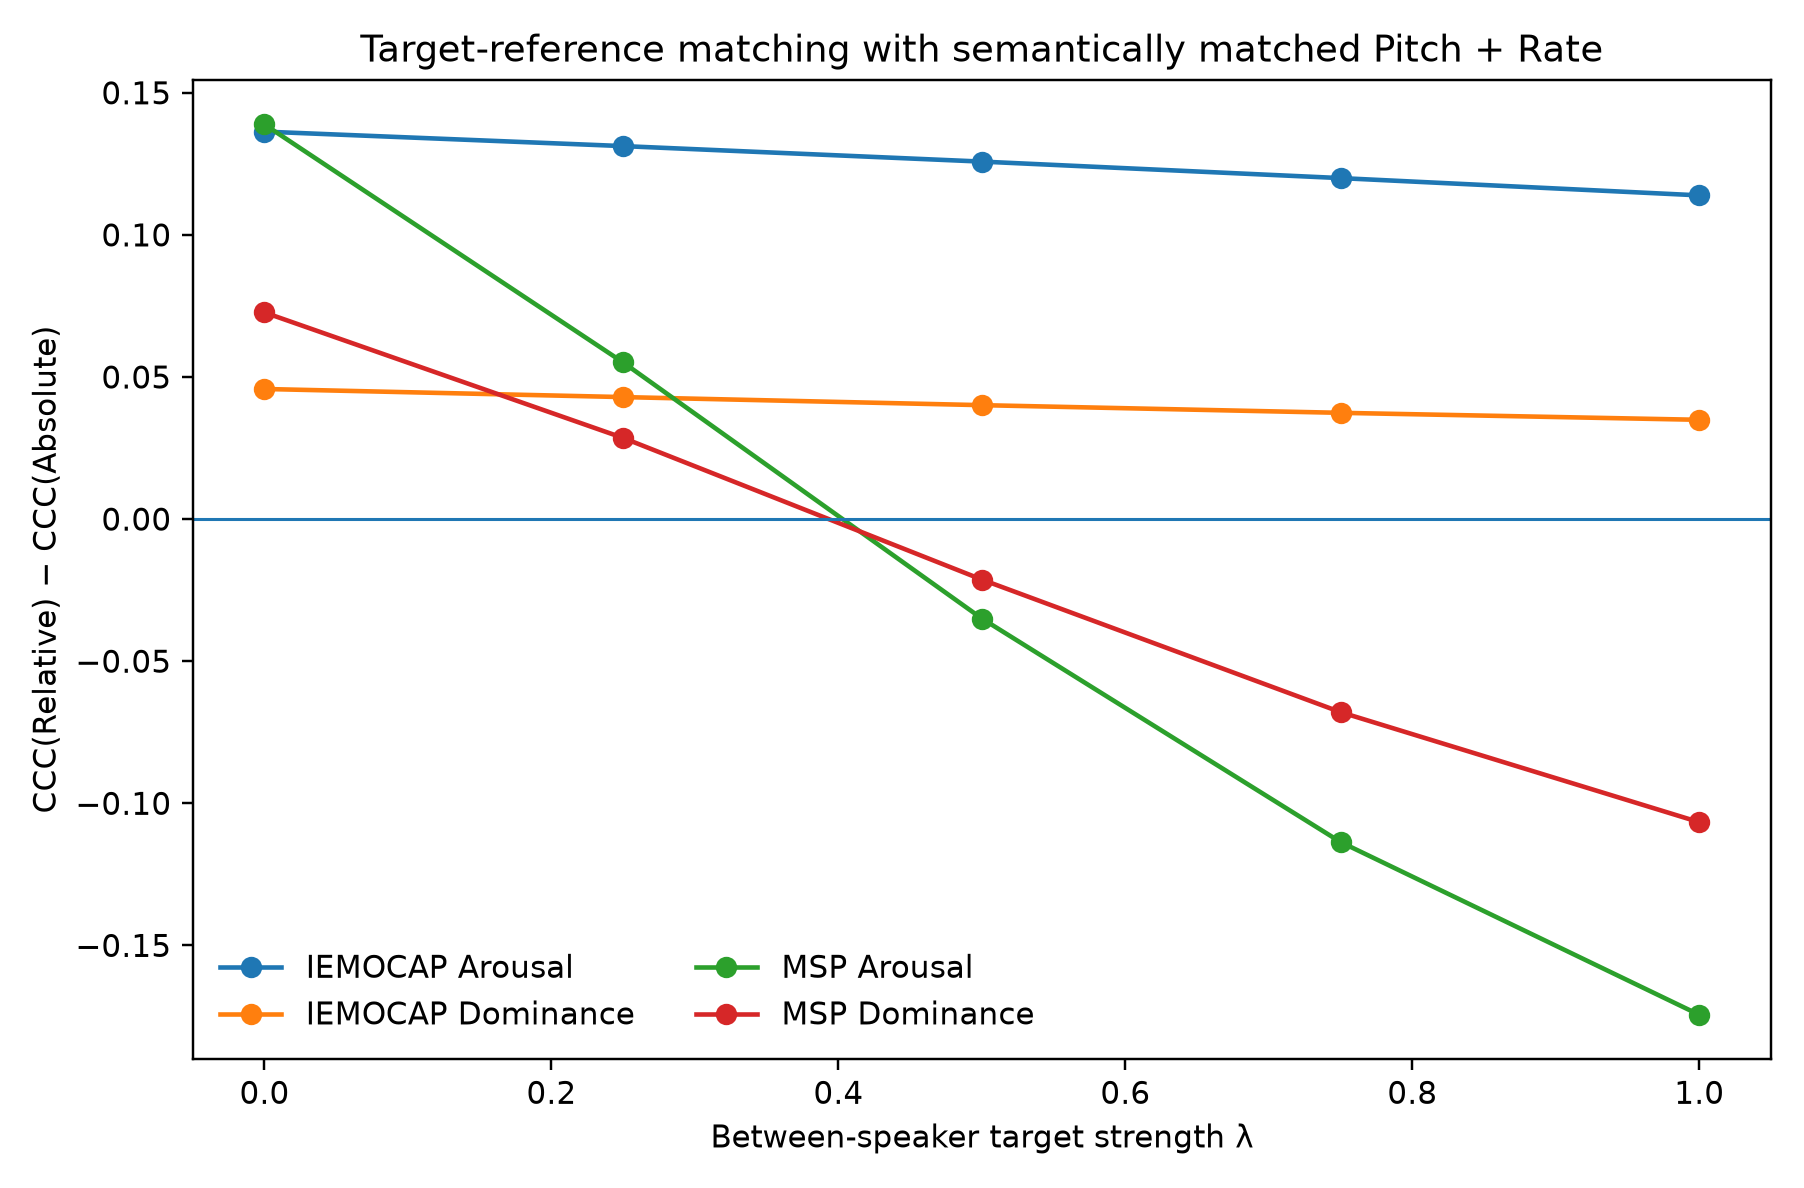
\includegraphics[width=\columnwidth]{figures/target_reference_matching.png}
    \caption{Controlled target-reference intervention with semantically matched Pitch+Rate features. As between-speaker target structure increases from the within-speaker endpoint toward the raw target, the Relative-minus-Absolute advantage decreases.}
    \label{fig:targetmatching}
\end{figure}

\begin{table}[t]
\centering
\small
\begin{tabular}{llrr}
\toprule
Corpus & Model/Target & Slope & 95\% CI\\
\midrule
MSP & Lin./A & -0.319 & [-0.338,-0.300]\\
MSP & Lin./D & -0.182 & [-0.197,-0.168]\\
MSP & Quad./A & -0.321 & [-0.341,-0.302]\\
MSP & Quad./D & -0.185 & [-0.200,-0.171]\\
IEMOCAP & Lin./A & -0.019 & [-0.066, 0.033]\\
IEMOCAP & Lin./D & -0.016 & [-0.048, 0.012]\\
IEMOCAP & Quad./A & -0.028 & [-0.076, 0.026]\\
IEMOCAP & Quad./D & -0.027 & [-0.062, 0.006]\\
\bottomrule
\end{tabular}
\caption{Slope of Relative-minus-Absolute CCC versus between-speaker target strength $\lambda$ for Pitch+Rate. Uncertainty resamples speakers. A/D denote Arousal/Dominance.}
\label{tab:crosscorpus}
\end{table}

\subsection{The effect strengthens with the full interpretable representation}

Combining all six validated prosodic attributes yields a particularly clear test on MSP (Table~\ref{tab:fullprosody}).
Relative-minus-Absolute slopes are about $-0.50$ for Arousal and $-0.41$ for Dominance under both model families, with narrow speaker-cluster intervals below zero.
At $\lambda=0$, Relative significantly outperforms Absolute in all four cells.
At $\lambda=1$, Hybrid significantly outperforms Relative in all four cells.
The mechanism is therefore not driven by one prosodic dimension or one linear decision surface.

\begin{table}[t]
\centering
\small
\setlength{\tabcolsep}{3pt}
\begin{tabular}{llrrr}
\toprule
Model & Target & R-A slope & R-A @0 & H-R @1\\
\midrule
Linear & Arousal & -0.502 & +0.190 & +0.359\\
Linear & Dominance & -0.404 & +0.142 & +0.294\\
Quadratic & Arousal & -0.507 & +0.182 & +0.376\\
Quadratic & Dominance & -0.409 & +0.136 & +0.311\\
\bottomrule
\end{tabular}
\caption{Full six-attribute MSP representation. R-A is Relative minus Absolute; H-R is Hybrid minus Relative. All displayed effects have speaker-cluster 95\% CIs excluding zero in the shown direction.}
\label{tab:fullprosody}
\end{table}

\subsection{Correct center identity is necessary}

The Hybrid result could in principle be a dimensionality effect.
The permutation intervention rules this out.
For raw MSP targets, true-center Hybrid exceeds mean permuted-center Hybrid by $+0.296$ CCC for Arousal and $+0.236$ for Dominance.
After the target is centered within speaker, these gaps collapse to approximately $+0.0014$ and $+0.0010$.
The useful information is therefore not an arbitrary vector with the distribution of speaker centers; it is the center associated with the correct speaker, and its utility depends on the target retaining speaker-level structure.

\subsection{Target-reference matching survives in WavLM space}

The mechanism also appears in learned speech representations.
Table~\ref{tab:wavlm} shows the IEMOCAP intervention when Absolute and Relative reference frames are constructed directly from frozen WavLM-large embeddings.
At layers 12 and 24, all four Arousal/Dominance Relative-minus-Absolute slopes are significantly negative under speaker-cluster bootstrap, despite the dataset having only ten speakers.
At $\lambda=0$, Relative significantly outperforms Absolute in all four layer-target cells; at the raw endpoint the preference reverses.

\begin{table}[t]
\centering
\small
\begin{tabular}{llrr}
\toprule
Layer & Target & R-A slope & R-A @0\\
\midrule
12 & Arousal & -0.083 & +0.040\\
12 & Dominance & -0.034 & +0.015\\
24 & Arousal & -0.096 & +0.047\\
24 & Dominance & -0.046 & +0.025\\
\bottomrule
\end{tabular}
\caption{Target-reference intervention in frozen WavLM-large embedding space on IEMOCAP. All slope and $\lambda=0$ confidence intervals exclude zero in the displayed direction.}
\label{tab:wavlm}
\end{table}

This distinction matters for interpretation.
The hand-engineered cross-corpus experiment is low-powered on IEMOCAP after correcting the independent resampling unit, whereas the high-dimensional learned representation yields a robust negative target-reference slope.
The shared qualitative mechanism is thus not tied to one manually chosen prosodic parameterization.

\begin{figure}[t]
    \centering
    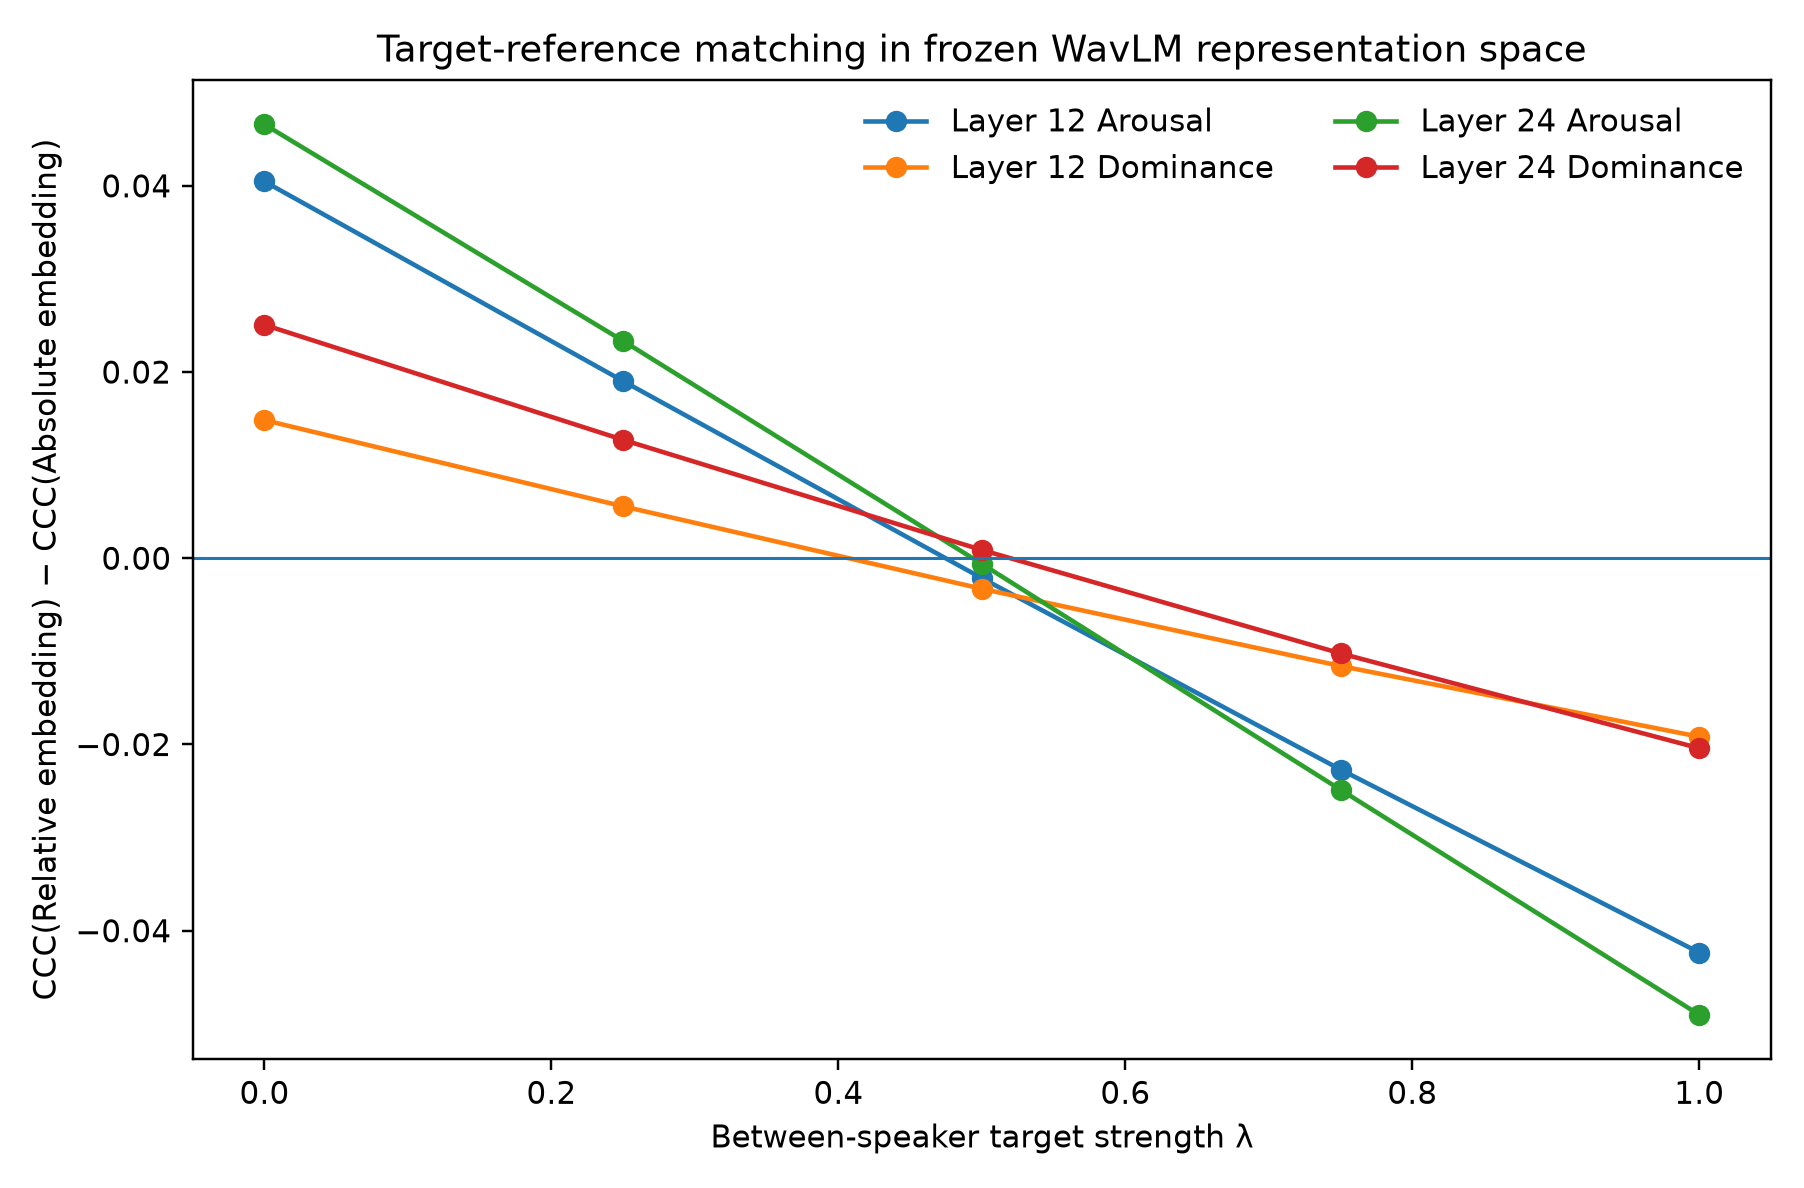
\includegraphics[width=\columnwidth]{figures/wavlm_target_reference.png}
    \caption{The same target-reference intervention in frozen WavLM-large embedding space on IEMOCAP. Speaker-relative embeddings are preferred near the within-speaker endpoint, while the preference shifts as stable between-speaker target structure is restored.}
    \label{fig:wavlmmatching}
\end{figure}

\subsection{Unlabeled enrollment recovers practical center utility}

The oracle analysis assumes access to a stable speaker center.
Table~\ref{tab:kshot} shows that this assumption can be relaxed.
With a fixed downstream pool, six-feature K-shot Hybrid already exceeds Absolute at $K=1$, and the gap grows with enrollment.
At $K=20$, Hybrid improves over Absolute by $+0.0390$ CCC for Arousal and $+0.0318$ for Dominance.
Increasing from $K=20$ to $K=50$ adds only $+0.0093$ and $+0.0074$ CCC, respectively.
At $K=50$, the remaining gap to the full-speaker oracle is only 0.0044 CCC for Arousal and 0.0037 for Dominance.

\begin{table}[t]
\centering
\small
\begin{tabular}{rrrrr}
\toprule
$K$ & A Abs. & A Hybrid & D Abs. & D Hybrid\\
\midrule
1  & .520 & .530 & .425 & .429\\
10 & .520 & .548 & .425 & .444\\
20 & .520 & .559 & .425 & .457\\
50 & .520 & .568 & .425 & .464\\
Oracle & --- & .572 & --- & .468\\
\bottomrule
\end{tabular}
\caption{Speaker-balanced CCC in the six-attribute fixed-pool unlabeled-enrollment experiment. The Absolute baseline is identical across K because downstream rows are fixed.}
\label{tab:kshot}
\end{table}

Center-estimation error decreases monotonically from $K=1$ to $K=50$ for all six attributes.
We therefore treat $K=20$ as a practical moderate-enrollment operating point, not a hard saturation boundary: the preregistered mean $K20\!\rightarrow\!K50$ gain is below 0.01 for both targets, but the Arousal confidence interval still extends slightly above 0.01.

\section{Discussion}

\subsection{Normalization is an information transformation}

Speaker normalization is often described as removing nuisance variability.
Our results suggest a more precise interpretation: normalization changes what information is directly available to the predictor.
Relative features emphasize within-speaker deviations and suppress stable speaker centers.
This is beneficial when the target is defined in the same within-speaker frame.
When the target retains stable between-speaker structure, removing the center can discard useful signal.

The Hybrid representation makes this decomposition explicit.
Its advantage on raw MSP Arousal/Dominance disappears when the appended center belongs to the wrong speaker and becomes nearly irrelevant after within-speaker target centering.
This supports a reference-matching mechanism rather than a generic benefit from additional dimensions.

\subsection{Reconciling invariance and personalization}

The reference-frame account provides a common explanation for two literatures that can otherwise appear contradictory.
Speaker-invariant methods are sensible when speaker variation is a domain nuisance relative to the desired target \citep{gat2022speaker}.
Personalization is sensible when stable speaker information helps define the target or calibrate its scale \citep{sridhar2022personalization,tran2023personalized,triantafyllopoulos2024enrolment}.
Neither strategy is universally correct.
The relevant question is which target the system is intended to predict: population-level affect, deviation from a person's own baseline, or a mixture of the two.

\subsection{Why Arousal and Dominance are clearer than Valence}

The proposed mechanism is strongest for Arousal and Dominance.
On MSP, both dimensions have substantial between-speaker structure and are predictable from simple speaker-level prosodic centers.
Valence is much weaker in this acoustic space.
This is a useful boundary rather than a failure to be hidden: a reference-frame mechanism can only exploit between-speaker structure that is represented in the chosen predictors.
Lexical, semantic, contextual, and multimodal information may define a different reference structure for Valence.

\subsection{What the WavLM result adds}

WavLM \citep{chen2022wavlm} is not explicitly trained to implement our acoustic decomposition.
Yet subtracting speaker embedding centers creates a Relative representation whose advantage changes systematically with target reference frame.
This suggests that modern SSL encoders retain overlapping state and trait information rather than becoming speaker-invariant in a binary sense.
The downstream question is not only whether speaker information is encoded, but whether a task readout uses an appropriate reference frame.

\subsection{Deployment implications}

The full-speaker center is a useful diagnostic oracle but an unrealistic deployment assumption.
The fixed-pool K-shot experiment narrows this gap without using affect labels.
Twenty unlabeled utterances already recover most of the practical Hybrid gain on MSP, and 50 utterances approach the marginal oracle closely.
This does not imply a universal value of K: our separate IEMOCAP WavLM enrollment experiment is less monotonic at very small K.
Enrollment requirements depend on corpus size, speaker variability, representation dimension, and target structure.

\section{Conclusion}

We studied speaker normalization as a reference-frame choice rather than a universally beneficial preprocessing operation.
Across explicit prosody, controlled target interventions, center-identity permutation, frozen WavLM embeddings, and unlabeled K-shot enrollment, one pattern recurs: speaker-relative information is advantageous when the target is within-speaker, while stable speaker-center information becomes useful as the target contains more between-speaker structure.
The practical implication is not always normalize or never normalize.
It is to make the target reference frame explicit and match the representation to it.

\section*{Limitations}

The study has several limitations.
First, the strongest large-speaker inference comes from MSP-Podcast; continuous-affect external validation is currently limited to IEMOCAP, which has only ten speakers and five dyadic sessions.
Accordingly, the hand-engineered IEMOCAP slopes should be interpreted as directionally consistent but low-powered, and strict session-disjoint sensitivity is heterogeneous.
Second, the six-attribute interpretable representation is intentionally low-dimensional.
Voice quality, detailed contours, lexical content, context, and multimodal signals may have different between/within-speaker decompositions.
Third, our target interpolation is a controlled statistical construction.
It identifies a mechanism inside observed datasets but does not imply that a natural application has a known scalar $\lambda$.
Fourth, K-shot enrollment reduces dependence on full-speaker oracle centers but does not solve reference estimation in all deployment conditions; enrollment quality and quantity are corpus dependent.
Fifth, the categorical gender probe relies on dataset-provided binary labels and is used only as a stable-trait diagnostic.
It should not be interpreted as a claim that gender is binary, purely acoustic, or reducible to a stable biological speaker property.
Finally, the study does not show that every affect dimension, corpus, language, or representation exhibits the same effect magnitude.

\section*{Ethical Considerations}

The work analyzes existing speech corpora and speaker-level variation.
Speaker normalization and personalization can interact with demographic attributes, identity, and fairness.
Our goal is not to infer sensitive traits for deployment.
Gender classification is used only as a diagnostic demonstrating that relative pitch removes stable information; the paper does not advocate gender recognition systems.
Practical personalized systems should minimize retained identity information, obtain appropriate consent for enrollment data, and evaluate whether speaker-specific calibration produces unequal errors across groups.
Any released supplementary material should follow the licenses and redistribution conditions of the source corpora.

\bibliography{references}

\appendix

\section{Additional State--Trait Results}

For the categorical motivation experiment, Relative-minus-Absolute pitch Macro-F1 changes are:
ESD emotion $+0.0908$ and gender $-0.1330$; MEAD emotion $+0.0904$ and gender $-0.3790$; RAVDESS emotion $+0.0586$ and gender $-0.2299$.
Speaker-ID decoding decreases much less than gender decoding, so we do not claim that low-dimensional Relative prosody removes speaker identity.

\section{Additional Robustness Notes}

The main MSP target-reference effect remains strongly negative under speaker-cluster resampling rather than fold-level uncertainty.
The WavLM result is numerically stable to replacing the default Ridge solver with high-precision LSQR; primary slopes change by less than $2\times10^{-6}$.
For IEMOCAP, we exclude a loudness claim because an available relative-dB field does not behave consistently with a physically reconstructed RMS-dB alternative.
These negative and sensitivity results motivate the narrower claim in the main paper.

\section{WavLM K-shot Reference Recovery}

Using unlabeled speaker enrollment directly in WavLM embedding space, $K=20$ preserves negative Relative-minus-Absolute slope means in all four layer-by-target cells, with three of four pure within-speaker endpoint effects positive.
At $K=50$, all four slope signs match the full-speaker oracle and three of four absolute slope gaps are at most 0.03.
Very small K is not uniformly reliable, so we describe moderate enrollment as a deployment result rather than claiming arbitrary few-shot stability.

\end{document}
